%Ukazka zaverecne zpravy
%Posledni zmena 02/2018, Martin Cadik

\documentclass[11pt,a4paper,oneside]{article}
\usepackage[utf8]{inputenc}
\usepackage{a4wide}
\usepackage{url}
\usepackage[breaklinks=true,hidelinks]{hyperref}
%\usepackage[chapter]{algorithm}
%\floatname{algorithm}{Alg.} 
\usepackage{ifpdf}
\ifpdf
\usepackage[pdftex]{graphicx}
\DeclareGraphicsExtensions{.pdf,.png,.gif,.jpg}
\else
\usepackage[final]{graphicx}
\DeclareGraphicsExtensions{.eps,.png,.gif,.jpg}
\fi 
\graphicspath{{fig/}}
\usepackage[export]{adjustbox}


% TODO Jak moc mám přepisovat ten článek.
% TODO jak moc chce popisovat tu implementaci
% TODO uživatelská studie - to mám ukázat metodu lidem a říct mi, která se jim
% líbí víc?

\begin{document}

\thispagestyle{empty}
\begin{center}
\vspace*{60mm}
{Semestrální projekt předmětu Výpočetní fotogragie -- závěrečná zpráva }\\
\smallskip
{\Large\bf Tone Mapping: implementace algoritmu Khan20}\\
\smallskip
{\it Milan Tichavský, \url{xticha09@fit.vut.cz}}\\
\vfill
{\bf Vedoucí práce:} {\it doc. Ing. Martin Čadík, Ph.D., \url{cadik@fit.vut.cz}} 
\hfill {Květen 2025}


\end{center}
\newpage


\section{Úvod}

Zařízení běžně používaná k zobrazování digitálního obsahu, jako jsou monitory,
televizory a tiskárny, nejsou schopna zobrazit celý dynamický rozsah světla
přítomného v reálném světě. Z tohoto důvodu existují metody pro převod obrazu s
vysokým dynamickým rozsahem (HDR) na standardní dynamický rozsah (SDR), aby bylo
možné jej správně vizualizovat na dostupných zařízeních. Tento proces se nazývá
"tone mapping".

Cílem této práce je implementace a analýza jednoho z moderních tone-mapping
algoritmů, konkrétně metody Khan20~\cite{Khan2020}, jako pluginu do Tone Mapping
Studia (TMS)~\cite{TMS2025}.

\section{Teoretické základy}

Pro pochopení tone-mappingu je nutné zmínit vlastnosti lidského vidění. Lidské
oko dokáže adaptivně vnímat velký rozsah jasových hodnot díky nelineárnímu
vnímání jasu a kontrastu. Algoritmy tone-mappingu se často inspirují těmito
vlastnostmi a snaží se přizpůsobit zobrazení tak, aby výsledný obraz působil
přirozeně.

\section{Popis algoritmu Khan20}

Algoritmus Khan20 je globální tone-mapping operátor (TMO), to znamená že pro
transformaci je využita monotónní neklesající mapovací funkce. 
Algoritmus je založený na transformaci obrazu pomocí funkce \textit{Perceptual
Quantizer (PQ)} a histogramu jasu. Schéma algoritmu je vidět na obrázku
\ref{fig:schema}.

\begin{figure}[htb]
  \begin{center}
    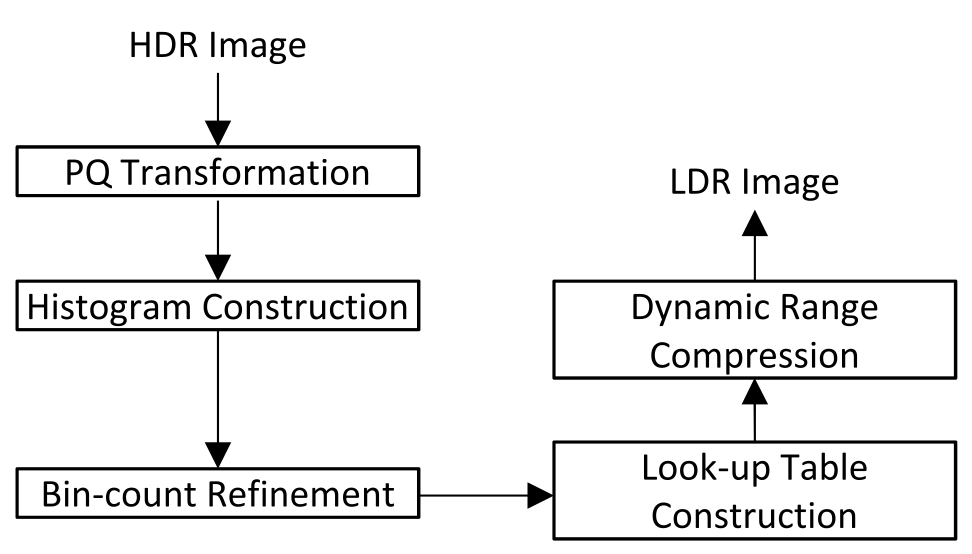
\includegraphics[width=0.8\linewidth]{fig/schema.png}
      \caption{Schéma algoritmu převzato z článku Khan20~\cite{Khan2020}.} 
    \label{fig:schema}
  \end{center}
\end{figure}

Funkce PQ vychází se snaží simulovat vnímaní lidského oka a transformuje
vstupní jas v rozsahu $[0, 10000]$ cd/m$^2$ na normalizovaný rozsah $[0,1]$,
přičemž nižší jasové hodnoty mají k dispozici větší relativní rozlišení.

Jak je vidět v tabulce \ref{tab:method-pq}, z takto transformovaného obrázku lze
jasně vidět celou scénu, která ale působí vybledle a má relativně nízký kontrast.

\begin{table}[htb]
    \centering
    \caption{Obrázky po transformaci funkcí \textit{Perceptual Quantizer}.}
    \label{tab:method-pq}
    \begin{tabular}{lll}
        \includegraphics[width=.33\linewidth,valign=m]{churchKhanPQ.png} &
        \includegraphics[width=.33\linewidth,valign=m]{buildingKhanPQ.png} &
        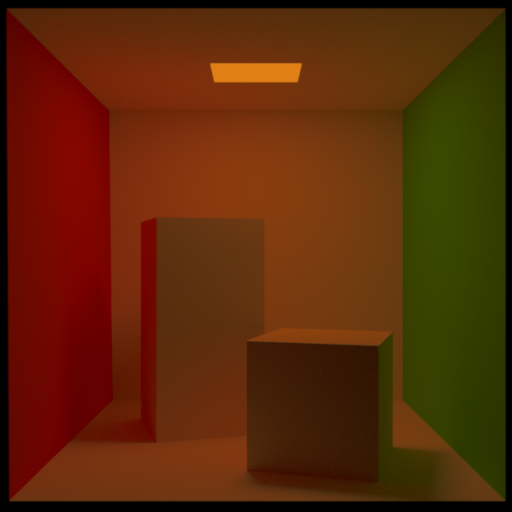
\includegraphics[width=.33\linewidth,valign=m]{cornell_boxKhanPQ.png} \\
    \end{tabular}
\end{table}

Z toho důvodu je nutné zkonstruovat histogram jasů, ze které je vytvořena
vyhledávací tabulka, podle které se provádí mapování každého vstupního pixelu.
Počet sloupců je dán parametrem $N$ (v příkazové řádce TMS lze zadat přepínačem
\texttt{-Bins}), přičemž implicitní hodnota je 256.

Už dříve bylo ukázáno, že použití klasického histogramu je problematické,
protože se může stát že malým oblastem bude přiřazeno až moc málo výsledného
rozsahu. Například pokud máme čistě modrou oblohu zabírající velkou část snímku,
nechceme, aby zabírala půlku výsledného rozsahu jasu. Proto je nutné
omezit počet pixelů v každém \textit{binu} pomocí parametru k, kde
$k/N*pixel\_count$ je maximální počet pixelů v daném sloupci. S pixelama které
se do daného počtu nevlezou se nic neděje, akorát pro další výpočty je počet
pixelů v daném sloupci podhonocen. V TMS lze nastavit přepínačem
\texttt{-Truncation} s implicitní hodnotou 5.

V článku samotném není přestě uvedeno, jakým způsobem se má obraz pomocí takto
transformovaných úrovní jasu převést do výsledného souboru. Proto jsem vstupní
obrázek převedl do Yxy barevného prostoru, nahradil jas (luminance) nově
vypočtenými hodnotami a tento obrázek uložil jako výsledek tone-mappingu.

\section{Výsledky}

% Nejdůležitější část -- diskuse výsledků, 
% načtené/vypozorované klady a zápory, operační složitost, ...
% Ukázkové obrázky.

V tabulce \ref{tab:method-comp} je vidět porovnání různých metod. Zvolil jsem ty
metody, které ve výchozím nastavení byly schopny rozumně zobrazit všechny tři
obrázky.

Jak je vidět, na všech obrázcích jsou scény krásně viditelné, bez toho aniž
bychom museli jakkoliv přenastavovat výchozí parametry. Hlavně v tom
se mi líbí algoritmus v porovnání s ostatními co jsem zkoušel, kde jsem
častokrát musel parametry měnit.

Subjektivně se mi víc líbí víc Drago03, protože jsou tmavé části opravdu tmavší
a barvy mi taky přijdou lepší. Například strop kostela je pro Khan20 hodně
v oranžovém odstínu. Na druhou stranu, světlejší barvy se hodí pro chodbu v
druhém obrázku, kde jsou více vidět detaily. Líbí se mi i záře kolem okna
kostela, které je jednoznačně nejsvítivějším místem celé scény.


\begin{table}[htb]
    \centering
    \caption{Srovnání různých metod; ve sloupcích zleva do prava jsou Khan20,
    Drago03 a Ward94. Všechny s výchozíma hodnotama parametrů v Tone Mapping
    Studiu.}
    \label{tab:method-comp}
    \begin{tabular}{lll}
        \includegraphics[width=.33\linewidth,valign=m]{churchKhan20.png} &
        \includegraphics[width=.33\linewidth,valign=m]{churchDrago03.png} &
        \includegraphics[width=.33\linewidth,valign=m]{churchWard94.png} \\
    \includegraphics[width=.33\linewidth,valign=m]{buildingKhan20.png} &
        \includegraphics[width=.33\linewidth,valign=m]{buildingDrago03.png} &
        \includegraphics[width=.33\linewidth,valign=m]{buildingWard94.png}\\
    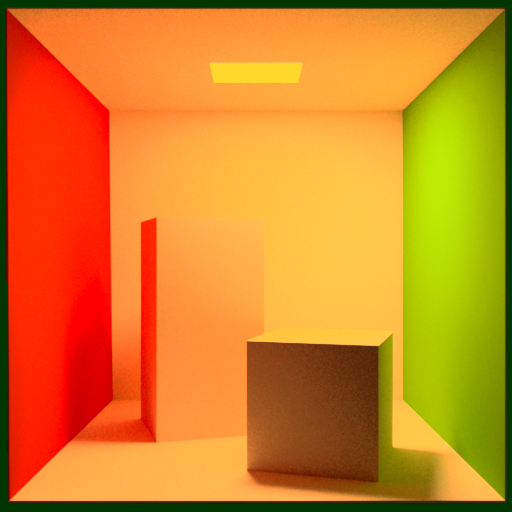
\includegraphics[width=.33\linewidth,valign=m]{cornell_boxKhan20.png} &
        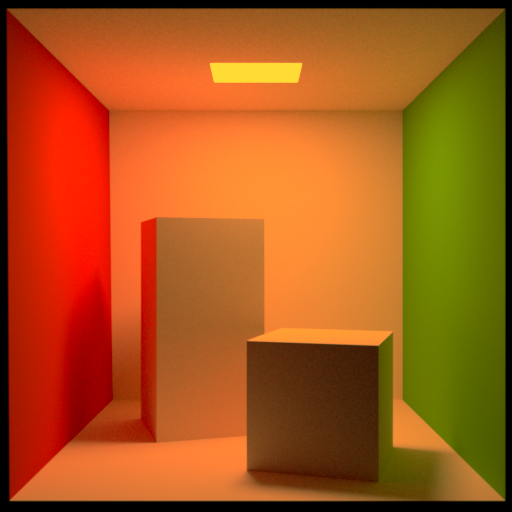
\includegraphics[width=.33\linewidth,valign=m]{cornell_boxDrago03.png} &
        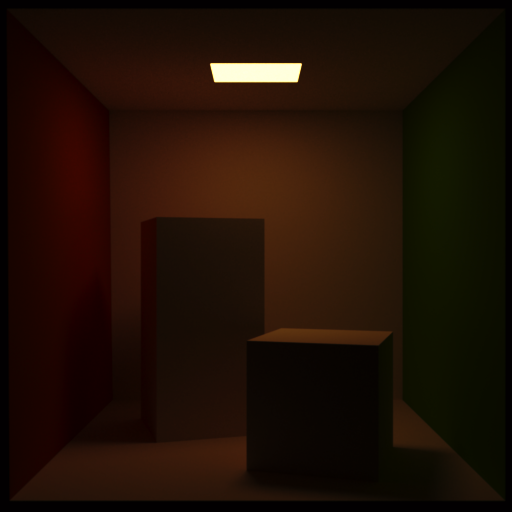
\includegraphics[width=.33\linewidth,valign=m]{cornell_boxWard94.png}\\
    \end{tabular}
\end{table}
Výpočetní složitost implementace je relativně nízká, program projde celkem 4x
přes všechny pixely obrázku a provede relativně jednoduché výpočty v každém
kroku. Počet průchodů by šel snížit, nicméně takto je kód podle mého názoru
přehlednější, kdy se každá funkce mapuje na jednu fázi algoritmu.

\section{Závěr}

V rámci projektu jsem implementoval plugin Khan20 do Tone Mapping studia a
porovnal jeho algoritmus s ostatními metodami. Výsledky ukazují, že algoritmus
funguje velmi dobře pro různé scény s výchozími parametry. Výstupní snímky jsou
o něco světlejší a možná méně saturované, než bych si přál z uměleckého
hlediska. Na druhou stranu metoda vyniká v zobrazování detailů, a to i v tmavých
oblastech. Díky tomu jsou detaily lépe viditelné i při odlescích na monitoru
nebo v přítomnosti silného externího osvětlení, což může být výhoda v různých
aplikacích.

\bibliographystyle{acm}
\bibliography{report}

\end{document}
